\chapter{权能表和权能管理}\label{ch:capability-table-management}

\section{权能的概念}\label{sec:2-capability-concept}

权能（Capability）是一种最早在多用户计算机系统中引入的用来控制访问权限的凭证\hyperref[cite:2-1]{{[}1{]}}。它是一种不可伪造的用来唯一标识某种资源以及允许对该资源所进行的操作的凭证。比如，Unix 的文件描述符就是一种权能\hyperref[cite:2-2]{{[}2{]}}；Windows 的访问权限也是一种权能。从某种意义上讲，权能就是一个指向某种资源的胖指针（Fat
Pointer）。

我们使用如下三条原则来保证系统的安全性\hyperref[cite:2-2]{{[}2{]}}：

\begin{enumerate}
\def\labelenumi{\arabic{enumi}.}
\item
  权能是不可伪造和不可在用户态擅自修改的；
\item
  进程只能用良好定义的授权接口获取权能；
\item
  权能只会被给予那些系统设计时负责管理该资源的进程。

  第三代微内核普遍采用权能的概念来管理资源。在 RME 中，所有的内核资源都是使用权能来管理的，并且权能全部位于内核空间中的权能表内。每个进程都对应一个权能表（Capability
  Table），在调用系统调用时，系统查找内核对象就是从该进程的权能表内查找的。每个权能都有一系列的操作标志位，如果某个权能拥有某个操作标志位，那么就可以通过这个权能对该内核对象做此种操作\hyperref[cite:2-3]{{[}3{]}}。绝大多数系统，如 seL4 等\hyperref[cite:2-5]{{[}5{]}}，都具有操作标志位。但是对于一些其他系统\footnote{如Composite等}，某种内核对象的操作只有一个，因此不需要单独的操作标志位\hyperref[cite:2-4]{{[}4{]}}。

  除了权能之外，还有另外一种称为访问控制列表（Access Control List，ACL）\hyperref[cite:2-6]{{[}6{]}}的方法。它也可以用来管理权限，但是其访问权限管理粒度较粗，而且表格很容易变得很大。它的优点是权能的授予和撤销相对简单\footnote{尤其是撤销操作}。

  在 RME 中，使用权能的概念，可以方便地实现自主访问控制（Discretionary Access
  Control，DAC）和强制访问控制（Mandatory Access
  Control，MAC），也能方便地构建起多级安全机制，并且根据最小特权的原则规划整个用户应用程序的设计。
\end{enumerate}

\section{权能表的操作和权能的状态}\label{sec:2-capability-table-operations-and-states}

权能表是一种用来存放权能的内核对象。在 RME 中它是一个线性数组，每个数组位置的大小都是固定的8个机器字，可以用来存放一个权能。在权能内部，记载着内核资源的确切类型、在内核内存中的确切位置\footnote{一个指向内核地址空间的指针}、权能的父权能、权能传递引用计数和权能的当前状态。此外，还有一个时间戳计数器用来在多核并行情况下用来保证权能的操作安定（Quiescence）。

\subsection{权能的类型}\label{subsec:2-capability-types}

在 RME 中，权能一共有8种类型\footnote{不包括空白权能}，如下表所示。关于相应类型权能的信息，请查看相应的章节作为参考。本章只讲述权能表权能相关的内容。

\begin{xltabular}{\textwidth}{@{}>{\hsize=0.8412\hsize\raggedright\arraybackslash}X>{\hsize=0.7467\hsize\raggedright\arraybackslash}X>{\hsize=1.4121\hsize\raggedright\arraybackslash}X@{}}
\caption{权能的类型}\label{tab:2-1-capability-types}\\
\toprule
权能类型号 & 权能类型 & 用途\tabularnewline
\endfirsthead
\toprule
权能类型号 & 权能类型 & 用途\tabularnewline
\midrule
\endhead
\bottomrule
\endlastfoot
RME\_CAP\_TYPE\_NOP & 空白权能 &
权能表的这个位置是空白权能。\tabularnewline
RME\_CAP\_TYPE\_KFN & 内核功能权能 &
调用特殊功能内核函数的必备权能。\tabularnewline
RME\_CAP\_TYPE\_KOM & 内核内存权能 &
使用一段内核内存创建内核对象的必备权能。\tabularnewline
RME\_CAP\_TYPE\_CPT & 权能表权能 &
指向一个权能表对象，可用来进行权能表管理。\tabularnewline
RME\_CAP\_TYPE\_PGT & 页目录权能 &
指向一个页目录对象，可用来进行内存管理。\tabularnewline
RME\_CAP\_TYPE\_PRC & 进程权能 &
指向一个进程对象，可用来进行进程管理。\tabularnewline
RME\_CAP\_TYPE\_THD & 线程权能 &
指向一个线程对象，可用来进行线程管理。\tabularnewline
RME\_CAP\_TYPE\_INV & 迁移调用权能 &
指向一个迁移调用对象，可用来进行同步迁移调用。\tabularnewline
RME\_CAP\_TYPE\_SIG & 信号端点权能 &
指向一个信号端点对象，可进行信号的发射和接收。\tabularnewline
\end{xltabular}

每种权能都代表着对该种内核对象做操作的权力，也代表着该内核对象能实现的功能。需要注意的是，指向权能表的权能\footnote{简称权能表权能}是系统的元权能，因为该权能具有修改权能表的权力，能够决定权能表的内容。

\subsection{权能的传递引用计数和父权能}\label{subsec:2-reference-count-and-parent-capability}

对于那些在创建内核对象过程中创建的权能，我们把它们称为根权能；对于那些被权能传递操作创建的权能，我们把它们称作叶权能。根权能的标志是其附加属性被设置为ROOT，而用来记载根权能的指针此时变为记载引用计数，在初始创建时该计数为0。

权能的传递引用计数和根权能是用来跟踪权能传递关系的。权能可以被从一个权能表被传递给另外一个权能表，此时我们把源权能称为父权能，把目标权能称为子权能。子权能的根权能指针要指向根权能，同时根权能的引用计数要增加1。也即，如果父权能是根权能，那么子权能的根权能指针指向父权能；如果父权能是叶权能，那么子权能的根权能指针等于父权能的根权能指针。值得注意的是，某些内核对象在互相引用时也会增加引用计数。

在移除权能时，要求叶权能以及对内核对象的全部引用先被移除，然后根权能才能被删除。\hyperref[cite:2-4]{{[}4{]}}

\subsection{权能的状态}\label{subsec:2-capability-states}

权能的状态有四种：空白、创建中，有效和冻结。这四种状态可以通过系统调用相互转换。

要创建一个权能，调用相应的内核对象创建函数，使用权能表权能指明所被操作的权能表\footnote{由于创建操作需要向权能表内部增加权能，修改了权能表，因此需要权能表权能；同理，销毁内核对象也需要权能表权能。}，指明需要创建的内核对象的内核虚拟内存地址和一些必要参数即可。此时，被指定的权能表的空白位会先被原子比较交换指令修改为``创建中''，待到创建成功，便会把状态修改为``有效''，否则仍然为``空白''并且返回相应的错误码。在创建权能时，如果要分配内核内存，那么还需要一个内核内存权能。关于内核内存权能，请参见下一章节的描述。

关于权能的回收有两种实现。一种实现是seL4和Fiasco.OC等系统的实现，它们支持操作系统级权能回收的操作，也即只支持删除操作，而在删除时会递归遍历整棵权能传递树，回收所有的被传递的权能。RME系统则采用另外一种实现，将权能移除和删除分成两个操作。操作系统不会做递归遍历回收的工作，这个工作必须由用户态完成。这样做的好处是不需要加入内核抢占点，但坏处则是用户必须跟踪每一次权能传递而自行负责权能回收。\hyperref[cite:2-4]{{[}4{]}}

要删除或移除一个权能，首先要冻结这个位置。冻结操作是通过权能冻结系统调用进行的。此时，被指定的权能表的有效位会被修改为``冻结''。如果冻结不成功，那么会返回相应的错误码。如果冻结成功，等到权能操作安定之后，即可调用函数将其删除/移除。其中，删除操作会在移除权能的同时，删除相应的内核对象本身；而移除则仅仅移除权能而不删除内核对象。权能被移除后，就会变回``空白''状态。对于叶权能，只能使用权能移除操作；对于根权能则只能使用对应于该内核对象的删除操作。

删除操作和移除操作还有行为上的细微区别。如果删除操作检测到内核对象因为仍然存在引用而无法被删除，那么它会解冻根权能并返回 RME\_ERR\_CPT\_REFCNT 以方便用户继续操作。如果用户需要删除，那么需要重新冻结根权能后再删除。删除操作在检测到因为其他原因无法被删除时不进行解冻操作。移除操作由于不检测内核对象的引用，即便操作无法进行也不会解冻叶权能。

\subsection{时间戳计数器与多核并行考量}\label{subsec:2-timestamp-counter-and-multicore-parallelism}

多核环境的执行绪是非常复杂的。内核有一些数据结构，不希望在这样的复杂操作中受到同时修改，它要求所有的操作都是原子的。因此，有两种解决方案：第一种解决方案是采用在每次操作都上锁的方法，第二种方法是在改变权能状态时采用原子操作。采用上锁的方案会引入额外的操作，速度较低，而且还会造成缓存行竞争。缓存行竞争指的是CPU1试图修改该缓存行，CPU2则试图查询该缓存行的状态，从而导致CPU2的缓存频繁失效，等效于大大降低了内存的访问速度，导致频繁的权能操作效率严重降低。采用原子操作的方案则较少有这些问题，但是会带来额外的实现难度。在 RME 中，我们采用后一种方法来实现多核并行。

RME 内核采用了大量的比较交换原子操作、原子自加操作构成的读-改-写操作来修改权能。内核还使用一个时间戳计数器来确保没有内核操作的冲突，比如正在一个CPU上使用的内核对象在另一个CPU上遭到删除等。

如果我们想要删除或移除权能，我们必须保证权能已经被冻结一段时间。我们把这段时间叫做权能安定时间。这段时间长度是可以在内核中被配置的。它要求被配置为至少比内核的最坏执行时间的两倍要长。这样，我们可以保证在删除或移除权能时，权能已经安定下来，也即所有CPU核上涉及到该权能的所有操作都已经完成，就不会有相互冲突的操作了。比如，CPU1正在试图删除权能A，CPU2则同时试图使用它。CPU2可能已经完成了操作的合法性检查，正在进行该操作，如果CPU1不经冻结直接删除权能，则可能影响CPU2的相应操作执行。每个权能内部的时间戳计数器就是为记录冻结时间而存在的。它会记下上次冻结操作开始进行的时间，保证在完全冻结之前不会开始移除或删除操作。

完整的权能状态转移图如下所示。在创建开始时，进行创建的CPU会对该空白槽位进行一个比较交换操作，标志着创建开始，该槽位被占用，直到创建完成为止才把该槽位标注成有效状态，从此时开始可以使用该权能；如果该权能没有被引用，在用毕后想要销毁，那么需要先将其冻结。刚创建的权能必须等待一个安定时间才能被冻结，被冻结的权能必须等待一个安定时间才能被移除或删除。

在删除或移除权能时，我们必须先完成所有的检查，确认该权能可以删除或移除，之后通过比较交换原子操作变更当前槽位的状态到空白来保证只有一个CPU核上的操作能够进行下去，最后再执行真正的后续操作，也即内核对象销毁（删除）或根权能解除引用（移除）。在 RME 中，删除或移除操作完成后，就可以立即开始新的创建操作。这样的原因是，RME 在修改槽位状态之前已经把后续操作所需的信息保存到了本地变量，在修改之后不再会访问该权能槽位，而是利用保存的信息进行后续操作。在 Composite\hyperref[cite:2-4]{{[}4{]}}中，在修改后仍然有可能在后续过程中使用到该槽位上的信息，因此在这里还要插入一个安定时间，防止这个位置被新创建的权能覆盖。

\begin{figure}[htbp]
    \centering
    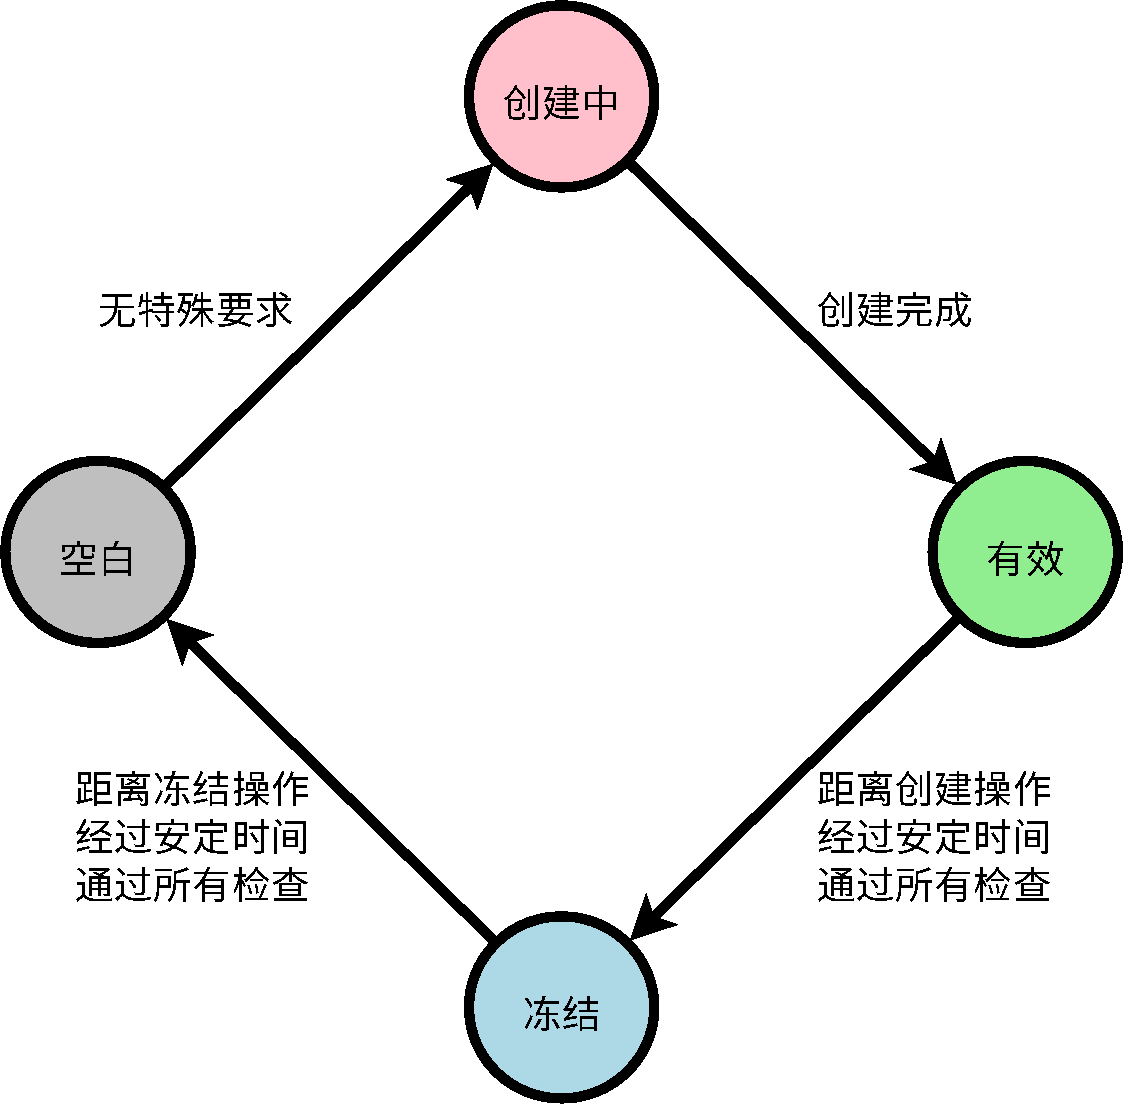
\includegraphics[width=0.72\textwidth]{Figure/image5.pdf}
    \caption{权能的生命周期}
    \label{fig:2-1-capability-lifecycle}
\end{figure}

安定时间要求至少是内核最坏执行时间两倍的原因如下：在调用权能冻结操作时，我们会先更新权能的时间戳，然后再通过原子操作标记该权能为被冻结。因此我们有如下的时间轴：

\begin{figure}[htbp]
    \centering
    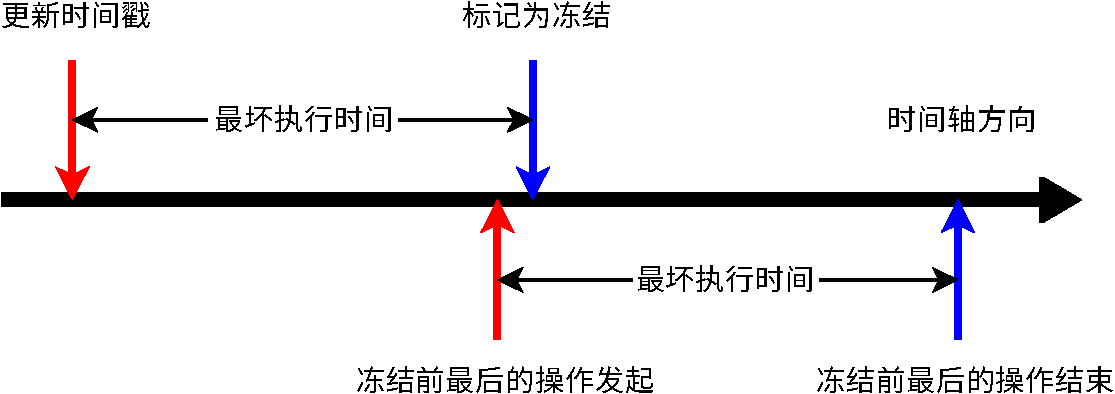
\includegraphics[width=0.72\textwidth]{Figure/image6.pdf}
    \caption{权能冻结的时间线}
    \label{fig:2-2-capability-freeze-timeline}
\end{figure}

从该时间轴中可以看出，从更新时间戳到冻结前的最后操作结束最多可能经过两个内核最坏执行时间。在实际使用中，推荐将安定时间至少配置为内核最坏执行时间的20倍\footnote{推荐高出一个数量级}，因为在工程中对最坏执行时间的估算往往只有数量级是准确的。

上面所说明的原理对于权能的创建------冻结安定时间也是一样的，在此不赘述。

\subsection{权能表结构}\label{subsec:2-capability-table-structure}

权能表可以被组织成多级结构。组织的具体方法是，在权能表内部放入权能表权能，这样权能表就可以组织成一个基数树。在对内核对象做操作时，需要传递一个权能号，指定这个权能在当前进程的权能表内部的位置。权能号最多可以编码两级查找。我们把一级查找可以达到的范围称为主权能表，把只有二级查找才能到达的范围称为扩展权能表。在32位系统下，权能号是一个16位的值；在64位系统下，权能号是一个32位的值。在更高位的系统下，依此类推。具体的编码方法如下：

\begin{xltabular}{\textwidth}{@{}>{\hsize=0.6388\hsize\raggedright\arraybackslash}X>{\hsize=0.7677\hsize\raggedright\arraybackslash}X>{\hsize=1.5935\hsize\raggedright\arraybackslash}X@{}}
\caption{权能号的编码方法}\label{tab:2-2-capability-number-encoding}\\
\toprule
系统位数 & 编码类型 & 编码方法\tabularnewline
\endfirsthead
\toprule
系统位数 & 编码类型 & 编码方法\tabularnewline
\midrule
\endhead
\bottomrule
\endlastfoot
\multirow{2}{*}{32位系统} & 一级查找编码 & {[}15:8{]}保留 {[}7{]}固定为0
{[}6:0{]}位置\tabularnewline
& 二级查找编码 & {[}15{]}保留 {[}14:8{]}子表位置 {[}7{]}固定为1
{[}6:0{]}在子表中的位置\tabularnewline
\multirow{2}{*}{64位系统} & 一级查找编码 & {[}32:16{]}保留 {[}15{]}固定为0
{[}14:0{]}位置\tabularnewline
& 二级查找编码 & {[}32{]}保留 {[}31:16{]}子表位置 {[}15{]}固定为1
{[}14:0{]}在子表中的位置\tabularnewline
\end{xltabular}

可以看出，在32位系统下，单个权能表中最多可以有2\textsuperscript{7}=128个权能，在64位系统下这一个值则为2\textsuperscript{15}=32768。在 RME 中这个值由宏 RME\_CID\_2L 代表。与 seL4 等系统不同，RME 的权能表不支持基于基数树的无限级别查找。也即，扩展权能表内的权能表权能指向的权能表\footnote{也即二级扩展权能表}中的权能，不被认为在扩展权能表之内，无法通过二级查找编码被直接使用\footnote{也即``我的附庸的附庸，不是我的附庸''}。如果要使用的话，必须通过权能传递调用传递到扩展权能表之内，才可以通过二级查找编码被调用。

如下图所示，在主权能表中有一个指向扩展权能表的权能表权能，它被放置在权能号4的位置上。该扩展权能表中的权能也可以通过二级查找编码访问。在该扩展权能表的权能号2的位置上有一个指向二级扩展权能表的权能表权能，该权能本身可以使用值为4:2的二级查找编码被访问，但它指向的二级扩展权能表中的权能则无法通过二级查找编码直接访问了。图中不能从主权能表被访问的部分以灰色表示。

\begin{figure}[htbp]
    \centering
    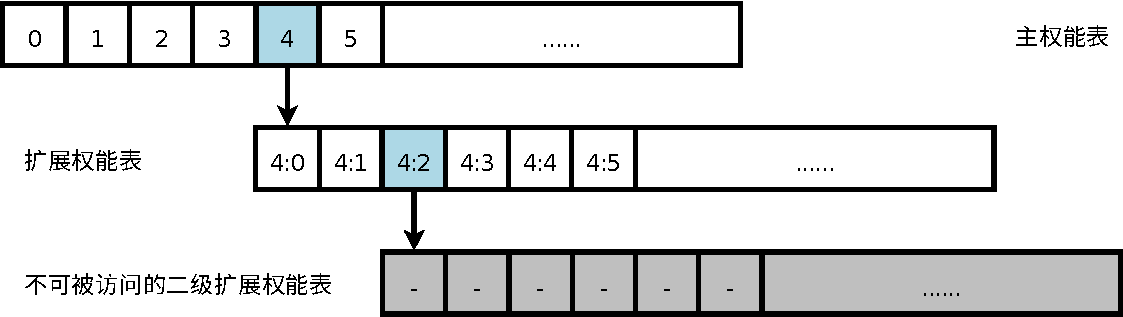
\includegraphics[width=0.72\textwidth]{Figure/image7.pdf}
    \caption{权能表结构图}
    \label{fig:2-3-capability-table-structure}
\end{figure}

\section{权能表功能列表}\label{sec:2-capability-table-function-list}

与权能表有关的内核功能如下：

\begin{xltabular}{\textwidth}{@{}>{\hsize=1.1605\hsize\raggedright\arraybackslash}X>{\hsize=0.8843\hsize\raggedright\arraybackslash}X>{\hsize=0.9552\hsize\raggedright\arraybackslash}X@{}}
\caption{权能表相关内核功能}\label{tab:2-3-capability-table-kernel-functions}\\
\toprule
调用号 & 类型 & 用途\tabularnewline
\endfirsthead
\toprule
调用号 & 类型 & 用途\tabularnewline
\midrule
\endhead
\bottomrule
\endlastfoot
RME\_SVC\_CPT\_CRT & 系统调用 & 创建权能表\tabularnewline
RME\_SVC\_CPT\_DEL & 系统调用 & 删除权能表\tabularnewline
RME\_SVC\_CPT\_ADD & 系统调用 & 权能传递\tabularnewline
RME\_SVC\_CPT\_FRZ & 系统调用 & 权能冻结\tabularnewline
RME\_SVC\_CPT\_REM & 系统调用 & 权能移除\tabularnewline
\end{xltabular}

权能表权能的操作标志如下：

\begin{xltabular}{\textwidth}{@{}>{\hsize=0.9567\hsize\raggedright\arraybackslash}X>{\hsize=0.6339\hsize\raggedright\arraybackslash}X>{\hsize=1.4095\hsize\raggedright\arraybackslash}X@{}}
\caption{权能表操作标志}\label{tab:2-4-capability-table-operation-flags}\\
\toprule
标志 & 位 & 用途\tabularnewline
\endfirsthead
\toprule
标志 & 位 & 用途\tabularnewline
\midrule
\endhead
\bottomrule
\endlastfoot
RME\_CPT\_FLAG\_CRT & {[}0{]} &
允许在该权能表中创建权能。\tabularnewline
RME\_CPT\_FLAG\_DEL & {[}1{]} &
允许删除该权能表中的权能。\tabularnewline
RME\_CPT\_FLAG\_FRZ & {[}2{]} &
允许冻结该权能表中的权能。\tabularnewline
RME\_CPT\_FLAG\_ADD\_SRC & {[}3{]} &
允许该权能表在权能传递作为来源表。\tabularnewline
RME\_CPT\_FLAG\_ADD\_DST & {[}4{]} &
允许该权能表在权能传递作为目标表。\tabularnewline
RME\_CPT\_FLAG\_REM & {[}5{]} &
允许移除该权能表中的权能。\tabularnewline
RME\_CPT\_FLAG\_PRC\_CRT & {[}6{]} &
允许在创建进程时将该权能表作为进程的权能表。\tabularnewline
RME\_CPT\_FLAG\_PRC\_CPT & {[}7{]} &
允许用该权能表替换某进程的权能表。\tabularnewline
\end{xltabular}

关于上表中的位{[}6{]}和位{[}7{]}，请参见\ref{subsec:4-create-a-process}
和\ref{subsec:4-change-process-capability-table}
。

\subsection{创建权能表}\label{subsec:2-create-a-capability-table}

该操作会创建一个权能表，并将其权能放入某个已存在的权能表。在权能表是一种内核对象，因此创建时需要指定其所使用的内核内存。在 RME 中，我们采用内核内存权能和内核起始相对虚拟地址的方法确定该内核对象的真实内核虚拟地址。每一个内核内存权能都会指定一个允许范围\footnote{由内核内存起始绝对虚拟地址和内核内存终止绝对虚拟地址组成}，只有这个范围内的内核内存才能在创建内核对象时使用。这个内核内存权能的内核起始绝对虚拟地址加上在创建内核对象时额外指定的内核起始相对虚拟地址（Relative
Address,
Raddr）才是内核对象的真实内核虚拟地址。这一点对于包括权能表在内的其他的内核对象都是相同的，在后面的章节中将不再赘述。关于内核内存权能的详细信息请参见\ref{sec:3-kernel-memory-function-list}
。

创建权能表操作需要如下几个参数：

\begin{xltabular}{\textwidth}{@{}>{\hsize=0.7639\hsize\raggedright\arraybackslash}X>{\hsize=0.6758\hsize\raggedright\arraybackslash}X>{\hsize=0.6758\hsize\raggedright\arraybackslash}X>{\hsize=1.8846\hsize\raggedright\arraybackslash}X@{}}
\caption{创建权能表的所需参数}\label{tab:2-5-create-capability-table-parameters}\\
\toprule
参数名称 & 类型 & 域 & 描述\tabularnewline
\endfirsthead
\toprule
参数名称 & 类型 & 域 & 描述\tabularnewline
\midrule
\endhead
\bottomrule
\endlastfoot
Svc\_Num & ptr\_t & N & 必须为 RME\_SVC\_CPT\_CRT。\tabularnewline
Cap\_Cpt\_Crt & cid\_t & C &
一个对应于必须拥有 RME\_CPT\_FLAG\_CRT 属性的权能表权能的权能号，该权能号对应的权能指向要接受此新创建的权能表权能的权能表。该权能号可以是一级或二级查找编码。\tabularnewline
Cap\_Kom & cid\_t & P1.D1 &
一个内核内存权能号，其标识的内核内存范围必须能够放下整个权能表，并且要拥有 RME\_KOM\_FLAG\_CPT 属性。该权能号可以是一级或二级查找编码。\tabularnewline
Cap\_Crt & cid\_t & P1.D0 &
一个对应于接受该新创建的权能表权能的权能表的某位置的权能号。该权能号对应的权能必须是空白的。该权能号只能是一级查找编码。\tabularnewline
Raddr & ptr\_t & P2 &
新创建的权能表要使用的内核起始相对虚拟地址。这个地址是相对于 Cap\_Kom 对应的内核权能的起始虚拟地址的。\tabularnewline
Entry\_Num & ptr\_t & P3 &
该权能表包含的表项数目，必须在 1 到 RME\_CID\_2L 之间。如果 RME\_CPT\_ENTRY\_MAX\footnote{见 7.3.2} 被定义为一个小于 RME\_CID\_2L 且不为 0 的值，则该数目必须在 1 到 RME\_CPT\_ENTRY\_MAX 之间。\tabularnewline
\end{xltabular}

该操作的返回值可能如下：

\begin{xltabular}{\textwidth}{@{}>{\hsize=0.7950\hsize\raggedright\arraybackslash}X>{\hsize=1.2050\hsize\raggedright\arraybackslash}X@{}}
\caption{创建权能表的可能返回值}\label{tab:2-6-create-capability-table-return-values}\\
\toprule
返回值 & 意义\tabularnewline
\endfirsthead
\toprule
返回值 & 意义\tabularnewline
\midrule
\endhead
\bottomrule
\endlastfoot
    0 & 操作成功。\tabularnewline
    RME\_ERR\_CPT\_RANGE & 传入的权能表权能数目参数超出了允许的范围。\tabularnewline
    RME\_ERR\_CPT\_RANGE & Cap\_Cpt\_Crt 的一级/二级查找超出了范围。\tabularnewline
    RME\_ERR\_CPT\_RANGE & Cap\_Kom 的一级/二级查找超出了范围。\tabularnewline
    RME\_ERR\_CPT\_RANGE & Cap\_Crt 的一级查找超出了范围。\tabularnewline
    RME\_ERR\_CPT\_FROZEN & Cap\_Cpt\_Crt 的一级/二级查找的权能已经被冻结。\tabularnewline
    RME\_ERR\_CPT\_FROZEN & Cap\_Kom 的一级/二级查找的权能已经被冻结。\tabularnewline
    RME\_ERR\_CPT\_FROZEN & Cap\_Crt 被冻结，或者其它核正在该处创建权能。\tabularnewline
    RME\_ERR\_CPT\_TYPE & Cap\_Cpt\_Crt 不是权能表权能。\tabularnewline
    RME\_ERR\_CPT\_TYPE & Cap\_Kom 不是内核内存权能。\tabularnewline
    RME\_ERR\_CPT\_FLAG & Cap\_Cpt\_Crt 无 RME\_CPT\_FLAG\_CRT 属性。\tabularnewline
    RME\_ERR\_CPT\_FLAG & Cap\_Kom 无 RME\_KOM\_FLAG\_CPT 属性，或范围错误。\tabularnewline
    RME\_ERR\_CPT\_EXIST & Cap\_Crt 不是空白权能。\tabularnewline
    RME\_ERR\_CPT\_KOT & 分配内核内存失败。\tabularnewline
\end{xltabular}

\subsection{删除权能表}\label{subsec:2-delete-a-capability-table}

该操作会删除一个权能表。被删除的权能表必须不含有权能，也即其全部权能位置应该都是空白的。删除权能表需要以下几个参数：

\begin{xltabular}{\textwidth}{@{}>{\hsize=0.7639\hsize\raggedright\arraybackslash}X>{\hsize=0.6758\hsize\raggedright\arraybackslash}X>{\hsize=0.6758\hsize\raggedright\arraybackslash}X>{\hsize=1.8846\hsize\raggedright\arraybackslash}X@{}}
\caption{删除权能表的所需参数}\label{tab:2-7-delete-capability-table-parameters}\\
\toprule
参数名称 & 类型 & 域 & 描述\tabularnewline
\endfirsthead
\toprule
参数名称 & 类型 & 域 & 描述\tabularnewline
\midrule
\endhead
\bottomrule
\endlastfoot
Svc\_Num & ptr\_t & N & 必须为 RME\_SVC\_CPT\_DEL。\tabularnewline
Cap\_Cpt\_Del & cid\_t & C &
一个对应于必须拥有 RME\_CPT\_FLAG\_DEL 属性的权能表权能的权能号，该权能号对应的权能指向含有正被删除的权能表权能的权能表。该权能号可以是一级或者二级查找编码。\tabularnewline
Cap\_Del & cid\_t & P1 &
一个对应于将被删除的权能表权能的权能号。该权能号对应的权能必须是一个权能表权能。该权能号只能是一级查找编码。\tabularnewline
\end{xltabular}

该操作的返回值可能如下：

\begin{xltabular}{\textwidth}{@{}>{\hsize=0.7450\hsize\raggedright\arraybackslash}X>{\hsize=1.2550\hsize\raggedright\arraybackslash}X@{}}
\caption{删除权能表的可能返回值}\label{tab:2-8-delete-capability-table-return-values}\\
\toprule
返回值 & 意义\tabularnewline
\endfirsthead
\toprule
返回值 & 意义\tabularnewline
\midrule
\endhead
\bottomrule
\endlastfoot
    0 & 操作成功。\tabularnewline
    RME\_ERR\_CPT\_RANGE & Cap\_Cpt\_Del 的一级/二级查找超出了范围。\tabularnewline
    RME\_ERR\_CPT\_RANGE & Cap\_Del 的一级查找超出了范围。\tabularnewline
    RME\_ERR\_CPT\_FROZEN & Cap\_Cpt\_Del 的一级/二级查找的权能已经被冻结。\tabularnewline
    RME\_ERR\_CPT\_FROZEN & Cap\_Del 未被冻结。\tabularnewline
    RME\_ERR\_CPT\_TYPE & Cap\_Cpt\_Del 不是权能表权能。\tabularnewline
    RME\_ERR\_CPT\_TYPE & Cap\_Del 不是权能表权能。\tabularnewline
    RME\_ERR\_CPT\_NULL & Cap\_Del 为空白权能。\tabularnewline
    RME\_ERR\_CPT\_NULL & 两个核同时试图删除该权能表，此时未成功的核返回该值。\tabularnewline
    RME\_ERR\_CPT\_FLAG & Cap\_Cpt\_Del 无 RME\_CPT\_FLAG\_DEL 属性。\tabularnewline
    RME\_ERR\_CPT\_QUIE & Cap\_Del 不安定。\tabularnewline
    RME\_ERR\_CPT\_EXIST & Cap\_Del 对应的权能表内还有权能。\tabularnewline
    RME\_ERR\_CPT\_REFCNT & Cap\_Del 的引用计数不为 0，或者不为根权能。\tabularnewline
\end{xltabular}

\subsection{权能传递}\label{subsec:2-transfer-a-capability}

该操作会将一个权能表中的某个权能传递到另外一个权能表的空白位置中。新创建的目标权能的父权能是源权能，并且源权能的引用计数会增加1。在权能表之间进行权能传递需要以下几个参数：

\begin{xltabular}{\textwidth}{@{}>{\hsize=0.7639\hsize\raggedright\arraybackslash}X>{\hsize=0.6758\hsize\raggedright\arraybackslash}X>{\hsize=0.6758\hsize\raggedright\arraybackslash}X>{\hsize=1.8846\hsize\raggedright\arraybackslash}X@{}}
\caption{权能传递的所需参数}\label{tab:2-9-capability-transfer-parameters}\\
\toprule
参数名称 & 类型 & 域 & 描述\tabularnewline
\endfirsthead
\toprule
参数名称 & 类型 & 域 & 描述\tabularnewline
\midrule
\endhead
\bottomrule
\endlastfoot
Svc\_Num & ptr\_t & N & 必须为 RME\_SVC\_CPT\_ADD。\tabularnewline
Cap\_Cpt\_Dst & cid\_t & P1.D1 &
一个对应于必须拥有 RME\_CPT\_FLAG\_ADD\_DST 属性的权能表权能的权能号，该权能号对应的权能指向目标权能表。该权能号可以是一级或者二级查找编码。\tabularnewline
Cap\_Dst & cid\_t & P1.D0 &
一个对应于将接受被传递的权能的权能号。该权能号对应的权能必须是空白的。该权能号只能是一级查找编码。\tabularnewline
Cap\_Cpt\_Src & cid\_t & P2.D1 &
一个对应于必须拥有 RME\_CPT\_FLAG\_ADD\_SRC 属性的权能表权能的权能号，该权能号对应的权能指向源权能表。该权能号可以是一级或者二级查找编码。\tabularnewline
Cap\_Src & cid\_t & P2.D0 &
一个对应于将传递的权能的权能号。该权能号对应的权能必须不为空白而且没有冻结。该权能号只能是一级查找编码。\tabularnewline
Flags & ptr\_t & P3 &
要传递的操作标志属性。只有这个操作标志允许的操作才能被新创建的权能执行。\tabularnewline
\end{xltabular}

需要注意的是，对于内核内存权能，其传递时还需要置于系统调用号 N 和权能表权能号 C 中的额外位来辅助确定其操作标志属性。具体的参数传递方法请参见\ref{sec:3-kernel-memory-function-list}
。

该操作的返回值可能如下：

\begin{xltabular}{\textwidth}{@{}>{\hsize=0.6791\hsize\raggedright\arraybackslash}X>{\hsize=1.3209\hsize\raggedright\arraybackslash}X@{}}
\caption{权能传递的可能返回值}\label{tab:2-10-capability-transfer-return-values}\\
\toprule
返回值 & 意义\tabularnewline
\endfirsthead
\toprule
返回值 & 意义\tabularnewline
\midrule
\endhead
\bottomrule
\endlastfoot
    0 & 操作成功。\tabularnewline
    RME\_ERR\_CPT\_RANGE & Cap\_Cpt\_Dst 或 Cap\_Cpt\_Src 的一级/二级查找超出了范围。\tabularnewline
    RME\_ERR\_CPT\_RANGE & Cap\_Dst 或 Cap\_Src 的一级查找超出了范围。\tabularnewline
    RME\_ERR\_CPT\_FROZEN & Cap\_Cpt\_Dst 或 Cap\_Cpt\_Src 的一级/二级查找的权能被冻结。\tabularnewline
    RME\_ERR\_CPT\_FROZEN & Cap\_Src 被冻结。\tabularnewline
    RME\_ERR\_CPT\_TYPE & Cap\_Cpt\_Dst 或 Cap\_Cpt\_Src 不是权能表权能。\tabularnewline
    RME\_ERR\_CPT\_NULL & Cap\_Src 为空白权能。\tabularnewline
    RME\_ERR\_CPT\_FLAG & Cap\_Cpt\_Src 无 RME\_CPT\_FLAG\_ADD\_SRC 属性。\tabularnewline
    RME\_ERR\_CPT\_FLAG & Cap\_Cpt\_Dst 无 RME\_CPT\_FLAG\_ADD\_DST 属性。\tabularnewline
    RME\_ERR\_CPT\_FLAG & Cap\_Src 的操作标志属性与传入的操作标志属性冲突，也即传入的属性包括了 Cap\_Src 不允许的操作或者操作范围。\tabularnewline
    RME\_ERR\_CPT\_FLAG & 传入的操作标志属性是不合法的，比如操作范围上下限冲突，或者不允许在传递产生的权能上做任何操作。\tabularnewline
    RME\_ERR\_CPT\_EXIST & Cap\_Dst 不是空白权能。\tabularnewline
    RME\_ERR\_CPT\_REFCNT & Cap\_Src 的引用计数超过了系统允许的最大范围。在 32 位系统中上限是 $2^{23}-1$，在 64 位系统中上限是 $2^{46}-1$。通常这是足够的。\tabularnewline
\end{xltabular}

\needspace{30\baselineskip}
\subsection{权能冻结}\label{subsec:2-freeze-a-capability}
\nopagebreak[4]

该操作会将一个权能表中的某个权能冻结。如果一个权能被冻结，那么在安定时间之后，能够保证从这个权能发起的，对这个权能指向的内核对象的操作在内核中全部停止，此时可以删除或移除该权能。注意，这并不等价于该权能指向的内核对象的全部操作都停止，因为还可能有其他权能指向这个内核对象，而从这些权能发起的内核对象操作仍然可以进行。如果根权能被冻结，那么才能保证该内核对象上的所有操作都停止，此时才可以删除该权能和内核对象。冻结权能操作也是由比较交换操作原子执行的；但它失败时我们知道一定有其他核成功帮助我们冻结了该权能，因此仍然返回成功。

\needspace{20\baselineskip}
冻结一个权能需要如下参数：

\begin{xltabular}{\textwidth}{@{}>{\hsize=0.7639\hsize\raggedright\arraybackslash}X>{\hsize=0.6758\hsize\raggedright\arraybackslash}X>{\hsize=0.6758\hsize\raggedright\arraybackslash}X>{\hsize=1.8846\hsize\raggedright\arraybackslash}X@{}}
\caption{权能冻结的所需参数}\label{tab:2-11-capability-freeze-parameters}\\
\toprule
参数名称 & 类型 & 域 & 描述\tabularnewline
\endfirsthead
\toprule
参数名称 & 类型 & 域 & 描述\tabularnewline
\midrule
\endhead
\bottomrule
\endlastfoot
Svc\_Num & ptr\_t & N & 必须为 RME\_SVC\_CPT\_FRZ。\tabularnewline
Cap\_Cpt\_Frz & cid\_t & C &
一个对应于必须拥有 RME\_CPT\_FLAG\_FRZ 属性的权能表权能的权能号，该权能号对应的权能指向含有正被冻结的权能的权能表。该权能号可以是一级或者二级查找编码。\tabularnewline
Cap\_Frz & cid\_t & P1 &
一个对应于将被冻结的权能的权能号。该权能号只能是一级查找编码。\tabularnewline
\end{xltabular}

该操作的返回值可能如下：

\begin{xltabular}{\textwidth}{@{}>{\hsize=0.7950\hsize\raggedright\arraybackslash}X>{\hsize=1.2050\hsize\raggedright\arraybackslash}X@{}}
\caption{权能冻结的可能返回值}\label{tab:2-12-capability-freeze-return-values}\\
\toprule
返回值 & 意义\tabularnewline
\endfirsthead
\toprule
返回值 & 意义\tabularnewline
\midrule
\endhead
\bottomrule
\endlastfoot
    0 & 操作成功。\tabularnewline
    RME\_ERR\_CPT\_RANGE & Cap\_Cpt\_Frz 的一级/二级查找超出了范围。\tabularnewline
    RME\_ERR\_CPT\_RANGE & Cap\_Frz 的一级查找超出了范围。\tabularnewline
    RME\_ERR\_CPT\_FROZEN & Cap\_Cpt\_Frz 的一级/二级查找的权能已经被冻结。\tabularnewline
    RME\_ERR\_CPT\_FROZEN & Cap\_Frz 已经被冻结，无需再次冻结，或者正在被创建。\tabularnewline
    RME\_ERR\_CPT\_TYPE & Cap\_Cpt\_Frz 不是权能表权能。\tabularnewline
    RME\_ERR\_CPT\_NULL & Cap\_Frz 为空白权能。\tabularnewline
    RME\_ERR\_CPT\_FLAG & Cap\_Cpt\_Frz 无 RME\_CPT\_FLAG\_FRZ 属性。\tabularnewline
    RME\_ERR\_CPT\_QUIE & Cap\_Frz 不安定。\tabularnewline
    RME\_ERR\_CPT\_REFCNT & Cap\_Frz 的引用计数不为 0。\tabularnewline
\end{xltabular}

\subsection{权能移除}\label{subsec:2-remove-a-capability}

该操作会将一个权能表中的某个权能移除。被移除的权能必须不是根权能\footnote{对根权能应当使用删除操作}。移除一个权能不会导致与之相关联的内核对象被移除，被移除的仅仅是权能本身\footnote{删除操作则只能对不被引用的根权能使用，并且会同时删除根权能和内核对象}。移除权能操作也是由比较交换操作原子执行的；但它失败时我们知道一定有其他核成功帮助我们移除了该权能，因此仍然返回成功。

移除一个权能需要如下参数：

\begin{xltabular}{\textwidth}{@{}>{\hsize=0.7639\hsize\raggedright\arraybackslash}X>{\hsize=0.6758\hsize\raggedright\arraybackslash}X>{\hsize=0.6758\hsize\raggedright\arraybackslash}X>{\hsize=1.8846\hsize\raggedright\arraybackslash}X@{}}
\caption{权能移除的所需参数}\label{tab:2-13-capability-removal-parameters}\\
\toprule
参数名称 & 类型 & 域 & 描述\tabularnewline
\endfirsthead
\toprule
参数名称 & 类型 & 域 & 描述\tabularnewline
\midrule
\endhead
\bottomrule
\endlastfoot
Svc\_Num & ptr\_t & N & 必须为 RME\_SVC\_CPT\_REM。\tabularnewline
Cap\_Cpt\_Rem & cid\_t & C &
一个对应于必须拥有 RME\_CPT\_FLAG\_REM 属性的权能表权能的权能号，该权能号对应的权能指向含有正被移除的权能的权能表。该权能号可以是一级或者二级查找编码。\tabularnewline
Cap\_Rem & cid\_t & P1 &
一个对应于将被移除的权能的权能号。该权能号只能是一级查找编码。\tabularnewline
\end{xltabular}

该操作的返回值可能如下：

\begin{xltabular}{\textwidth}{@{}>{\hsize=0.7554\hsize\raggedright\arraybackslash}X>{\hsize=1.2446\hsize\raggedright\arraybackslash}X@{}}
\caption{权能移除的可能返回值}\label{tab:2-14-capability-removal-return-values}\\
\toprule
返回值 & 意义\tabularnewline
\endfirsthead
\toprule
返回值 & 意义\tabularnewline
\midrule
\endhead
\bottomrule
\endlastfoot
    0 & 操作成功。\tabularnewline
    RME\_ERR\_CPT\_RANGE & Cap\_Cpt\_Rem 的一级/二级查找超出了范围。\tabularnewline
    RME\_ERR\_CPT\_RANGE & Cap\_Rem 的一级查找超出了范围。\tabularnewline
    RME\_ERR\_CPT\_FROZEN & Cap\_Cpt\_Rem 的一级/二级查找的权能已经被冻结。\tabularnewline
    RME\_ERR\_CPT\_FROZEN & Cap\_Rem 未被冻结。\tabularnewline
    RME\_ERR\_CPT\_TYPE & Cap\_Cpt\_Rem 不是权能表权能。\tabularnewline
    RME\_ERR\_CPT\_NULL & Cap\_Rem 为空白权能。\tabularnewline
    RME\_ERR\_CPT\_NULL & 两个核同时试图移除该权能，此时未成功的核返回该值。\tabularnewline
    RME\_ERR\_CPT\_FLAG & Cap\_Cpt\_Rem 无 RME\_CPT\_FLAG\_REM 属性。\tabularnewline
    RME\_ERR\_CPT\_QUIE & Cap\_Rem 不安定。\tabularnewline
    RME\_ERR\_CPT\_ROOT & Cap\_Rem 为根权能，不能使用移除，请使用删除操作。\tabularnewline
\end{xltabular}

\section{本章参考文献}\label{sec:2-chapter-bibliography}

\protect\phantomsection\label{cite:2-1}

\noindent {[}1{]} J. B. Dennis and E. C. Van Horn, ``Programming semantics for multiprogrammed computations,'' \textit{Communications of the ACM}, vol. 9, pp. 143--155, 1966.

\protect\phantomsection\label{cite:2-2}

\noindent {[}2{]} J. S. Shapiro, J. M. Smith, and D. J. Farber, \textit{EROS: A Fast Capability System}, vol. 33. ACM, 1999.

\protect\phantomsection\label{cite:2-3}

\noindent {[}3{]} R. J. Feiertag and P. G. Neumann, ``The foundations of a provably secure operating system (PSOS),'' in \textit{Proceedings of the National Computer Conference}, 1979, pp. 329--334.

\protect\phantomsection\label{cite:2-4}

\noindent {[}4{]} Q. Wang, Y. Ren, M. Scaperoth, and G. Parmer, ``Speck: a kernel for scalable predictability,'' in \textit{Proceedings of the IEEE Real-Time and Embedded Technology and Applications Symposium (RTAS)}, 2015, pp. 121--132.

\protect\phantomsection\label{cite:2-5}

\noindent {[}5{]} G. Klein, K. Elphinstone, G. Heiser, J. Andronick, D. Cock, P. Derrin, et al., ``seL4: formal verification of an OS kernel,'' in \textit{Proceedings of the ACM SIGOPS 22nd Symposium on Operating Systems Principles}, Big Sky, MT, USA, 2009.

\protect\phantomsection\label{cite:2-6}

\noindent {[}6{]} B. W. Lampson, ``Protection,'' \textit{ACM SIGOPS Operating Systems Review}, vol. 8, pp. 18--24, 1974.

